\subsection{A tutorial on hidden Markov models and selected applications in speech recognition \cite{Rabiner1989A}}

This paper is a very classic and comprehensive tutorial on \emph{Hidden Markov Models (HMMs)}. Although HMMs is not among the deep learning approaches that emerged in recent years, the concepts behind HMMs are closely related to that of the \emph{Recurrent Neural Networks (RNNs)}.

\begin{figure}[htbp]
  \centering
  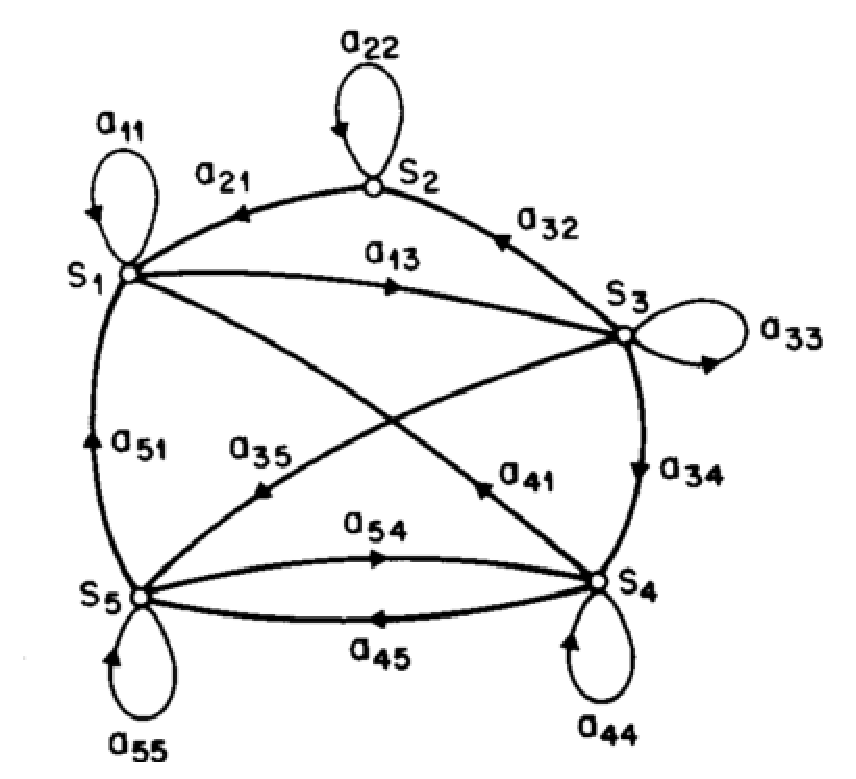
\includegraphics[width=.6\linewidth]{8_29_HMM_chain}\\
  \caption{A Markov chain with 5 states}\label{fig:chain}
\end{figure}

In the discrete Markov processes (without hidden states), a system at any time is described as being in one of a set of distinct state (cf. Figure \ref{fig:chain}). A full probabilistic description of the above system would require specification of the current state, as well as all the predecessor states. For the special case of a discrete, first order, Markov chain, it is assumed that the probabilistic description only depends on the current state and its immediate predecessor. This stochastic process is also called an observable Markov model, since the output of the process is the set of states at each instant of time, where each state corresponds to a physical (observable) event.

HMMs extend the concept to include the case where the observation is a probabilistic function of the hidden states, i.e., the resulting model is a doubly embedded stochastic process with an underlying stochastic process that is not observable, but can only be observed through another set of stochastic processed that produce the observations.

It would be better to explain the concept with the following example. Suppose on the other side of the curtain a person is performing a coin tossing experiment. That person will not tell you anything about what he is doing exactly (he may be tossing 2 or 3 different coins with different biased coins); he will only tell you the result of each coin flip (the observation).

\begin{figure}[htbp]
  \centering
  \subfigure{
    \label{fig:topka} %% label for first subfigure
    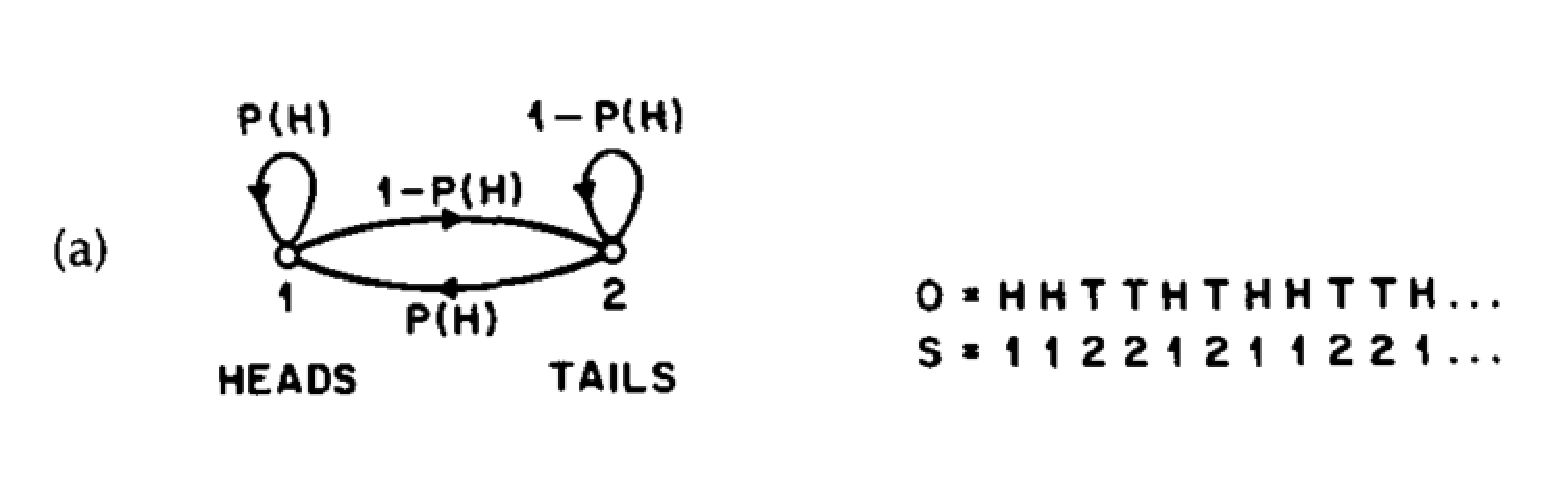
\includegraphics[width=2.2in]{8_29_HMM_coinA}}
  \subfigure{
    \label{fig:topkb} %% label for second subfigure
    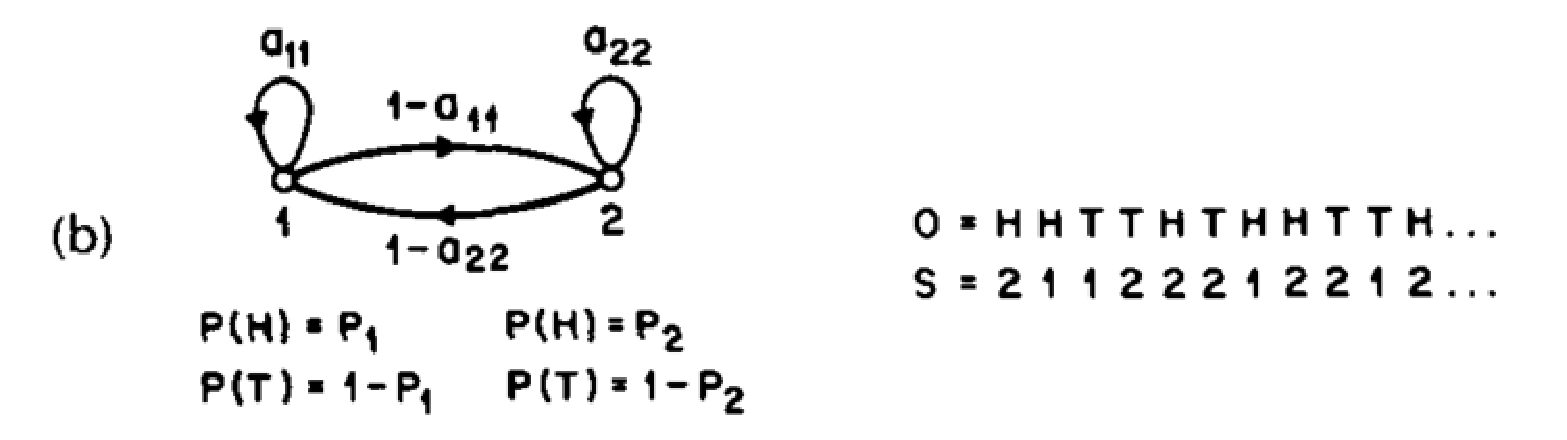
\includegraphics[width=2.2in]{8_29_HMM_coinB}}
  \subfigure{
    \label{fig:topkb} %% label for second subfigure
    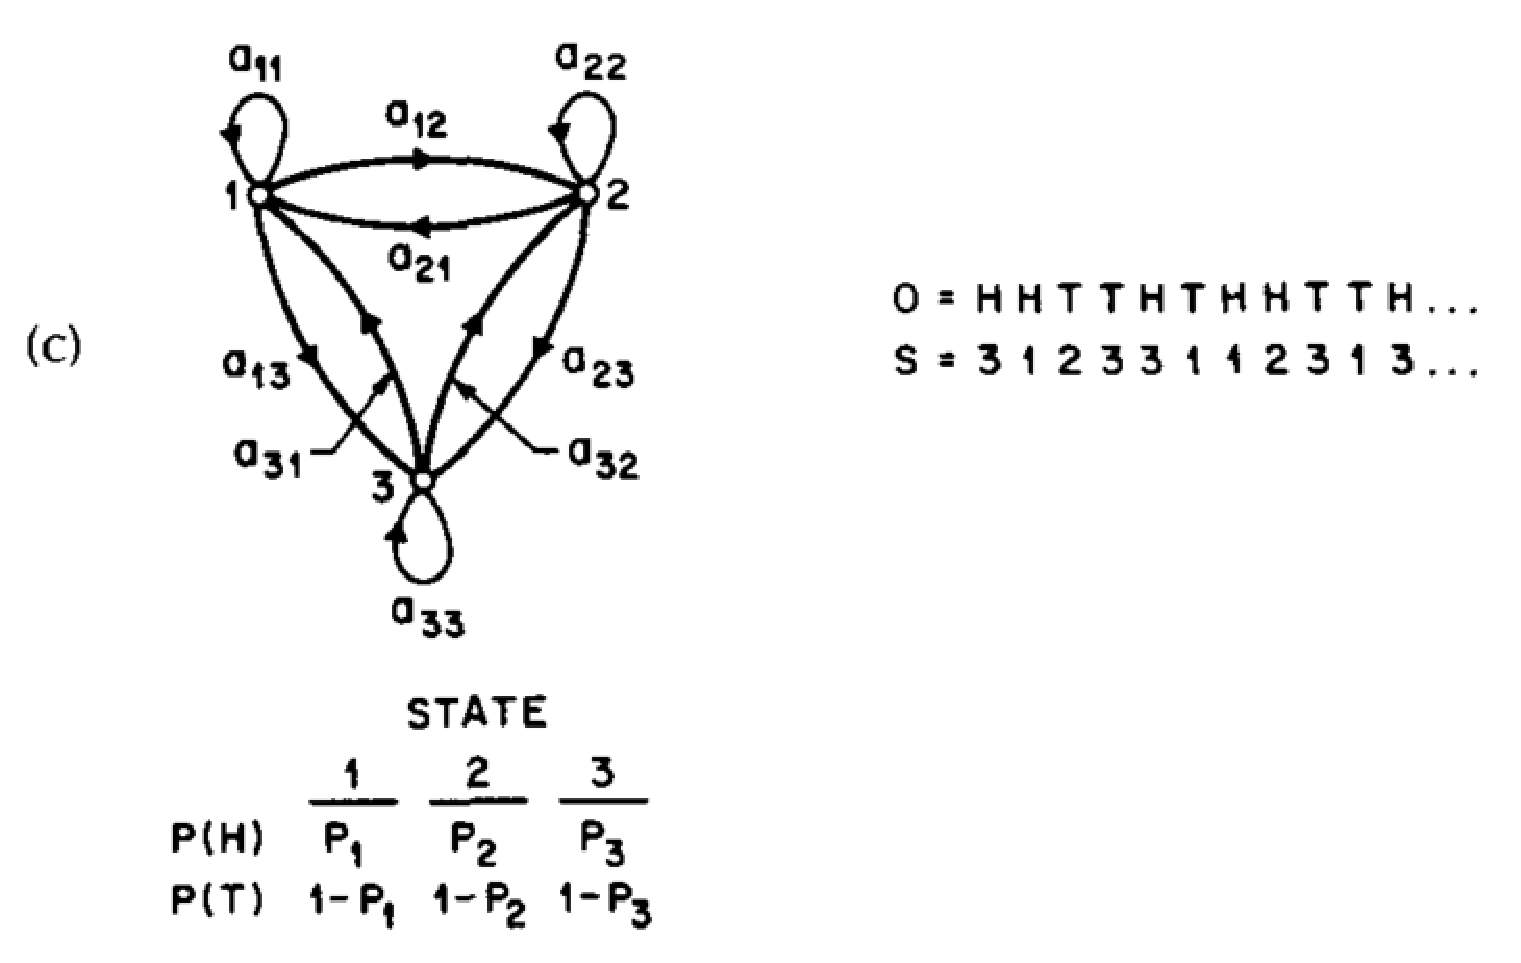
\includegraphics[width=2.2in]{8_29_HMM_coinC}}
  \caption{Three possible Markov models that can account for the results of hidden coin tossing experiments}\label{fig:coin}
\end{figure}

One possible choice would be to assume that only a single coin was being tossed. In this case the situation could be model with a 2-state (fully observable) model where each state corresponds to a side of the coin (cf. Figure \ref{fig:coin} (a)). We can also assume that two different biased coins were being tossed, and use the HMM in Figure \ref{fig:coin} (b) to describe this situation. Here each state corresponds to a different coin. Each state is characterized by a probability distribution of heads and tails, and transitions between states are characterized by a state transition matrix. We could further assume that there are 3 different coins, and model the system as a HMM with 3 hidden states (cf. Figure \ref{fig:coin} (c)).

An HMM is mathematically characterized by the following parameters: 1) $N$, the number of states in the model; 2) $M$, the number of distinct observation symbols; 3) The state transition probability distribution $A=\{a_{ij}\}$; 4) The observation symbol probability distribution in state $j$, $B = \{b_j(k)\}$; 5) The initial state distribution $\pi$. The paper uses the compact notation $\lambda = (A, B, \pi)$ to indicate the complete parameter set of the models.

There are three basic problems for HMMs: 1) How to efficiently compute $P(O| \lambda)$, the probability of the observation sequence given the model; 2) Given the observation sequence $O$ and the model $\lambda$, how to choose a corresponding state sequence $Q$ that is optimal; 3) How to adjust (or train) the parameters in $\lambda$ to maximize $P(O| \lambda)$.

The paper shows that all the three problems can be solved by the \emph{forward-backward procedure}. The basic idea of the forward-backward procedure is to apply the technique of dynamic programming. It introduces a forward variable $\alpha_t(i)$, which is probability of the partial observation sequence $O_1, ..., O_t$ (until time $t$) and state $S_i$ at time $t$. It shows how $\alpha_{t+1}(i)$ can be computed based on $\alpha_t(i)$ (the idea of dynamic programming). Similarly, a backward variable $\beta_t(i)$ is defined as the probability of the partial observation sequence from $t+1$ to the end. Finally, all the three problems can be solve by using the forward and backward variables.

In the remaining parts of the paper, it introduces various types of HMMs that have been previously studied (for example HMMs whose states are not fully connected). It also discusses the issues that arise in implementations, such as initial parameter estimates, model size, missing data, etc. Finally it describes some successful applications of HMMs in the field of speech recognizer. 